\section{Appendix}
\label{sec:appendix}
\subsection{Figure in Results: A ``distance-angle'' radar chart divided every 40cm within the range of 0 to 400cm}

\begin{figure}[H]
  \centering
  \begin{subfigure}[b]{0.3\linewidth}
    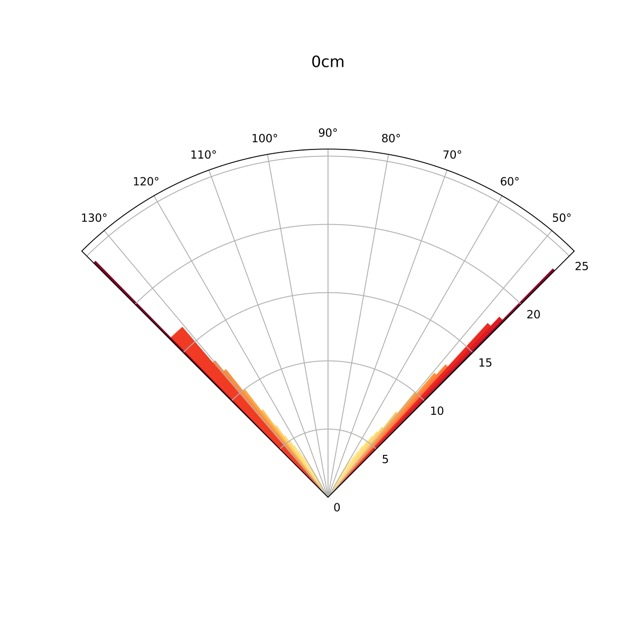
\includegraphics[width=\linewidth]{../Photos/angle-distance/0cm Medium}
  \end{subfigure}
  \hfill
  \begin{subfigure}[b]{0.3\linewidth}
    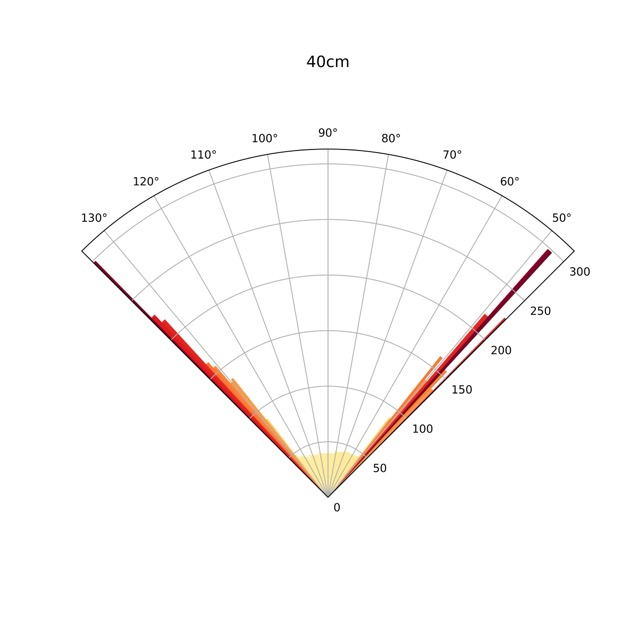
\includegraphics[width=\linewidth]{../Photos/angle-distance/40cm Medium}
  \end{subfigure}
  \hfill
  \begin{subfigure}[b]{0.3\linewidth}
    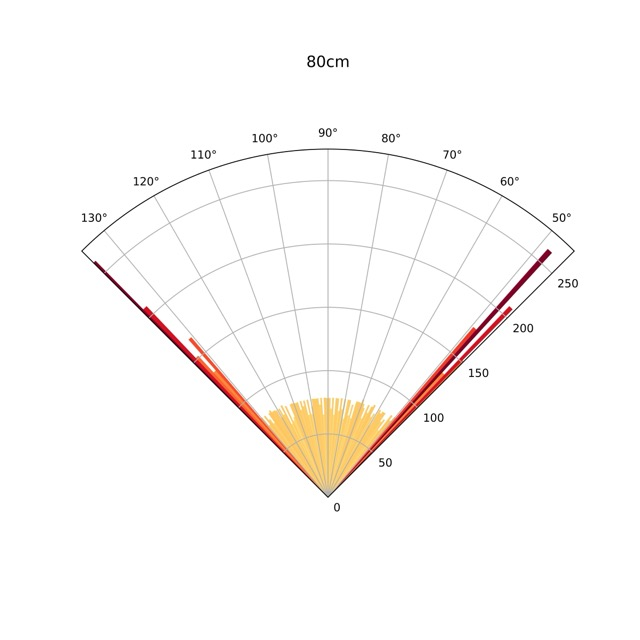
\includegraphics[width=\linewidth]{../Photos/angle-distance/80cm Medium}
  \end{subfigure}
  \label{fig:distance-angle1}
\end{figure}

\begin{figure}[H]
  \begin{subfigure}[b]{0.3\linewidth}
    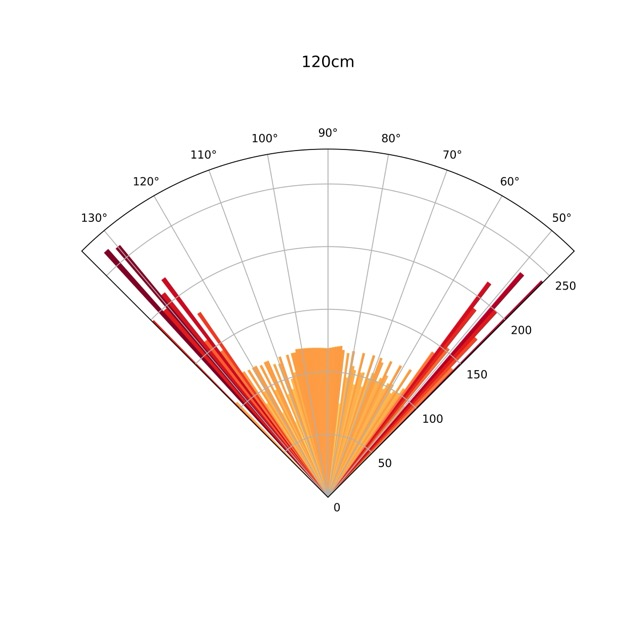
\includegraphics[width=\linewidth]{../Photos/angle-distance/120cm Medium}
  \end{subfigure}
  \hfill
  \begin{subfigure}[b]{0.3\linewidth}
    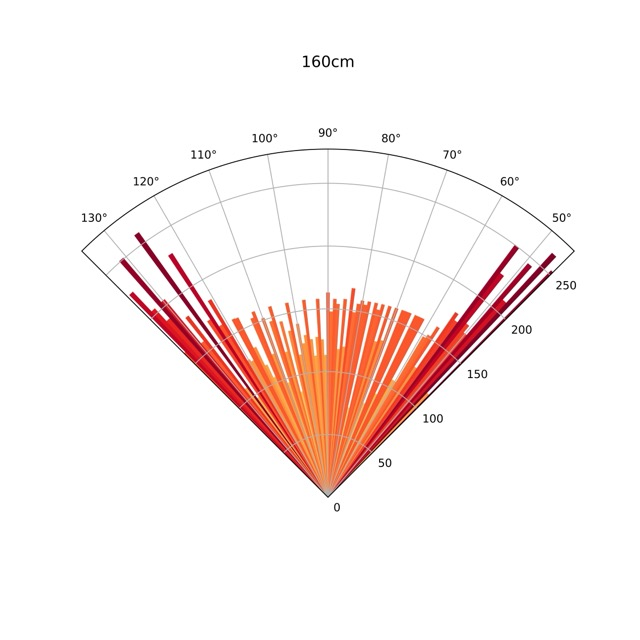
\includegraphics[width=\linewidth]{../Photos/angle-distance/160cm Medium}
  \end{subfigure}
  \hfill
  \begin{subfigure}[b]{0.3\linewidth}
    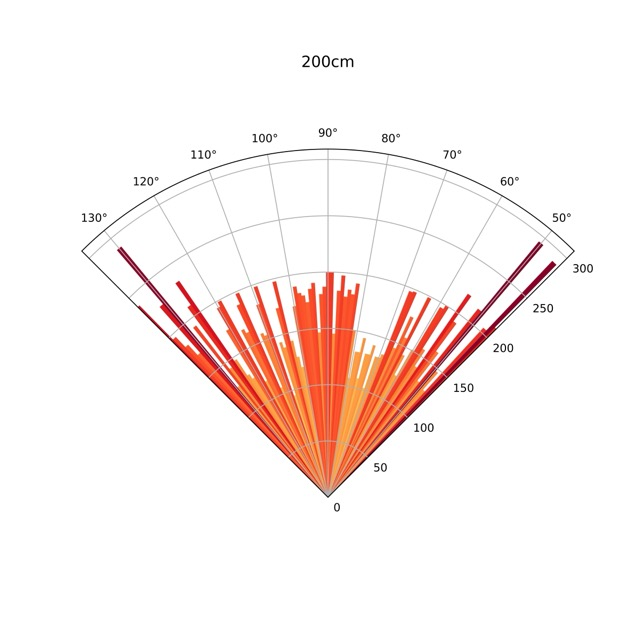
\includegraphics[width=\linewidth]{../Photos/angle-distance/200cm Medium}
  \end{subfigure}
  \label{fig:distance-angle2}
\end{figure}

\begin{figure}[H]
  \begin{subfigure}[b]{0.3\linewidth}
    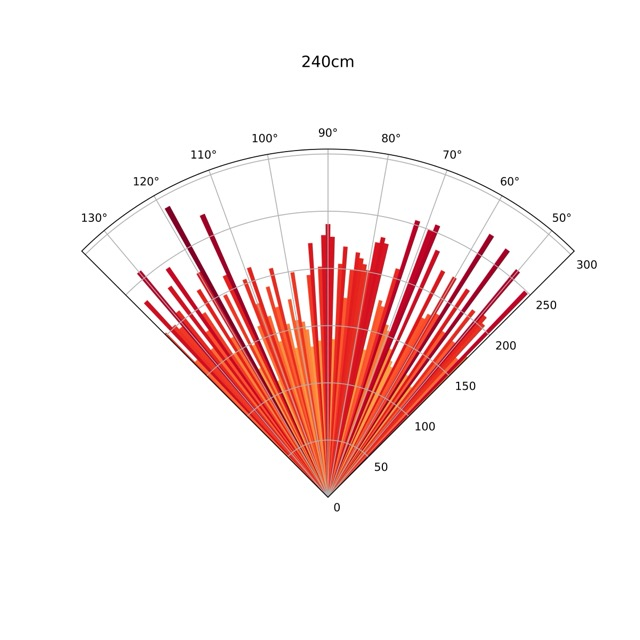
\includegraphics[width=\linewidth]{../Photos/angle-distance/240cm Medium}
  \end{subfigure}
  \hfill
  \begin{subfigure}[b]{0.3\linewidth}
    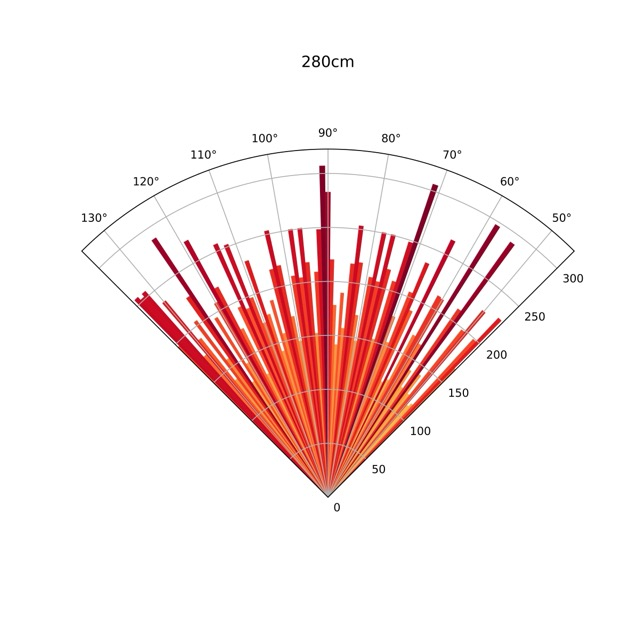
\includegraphics[width=\linewidth]{../Photos/angle-distance/280cm Medium}
  \end{subfigure}
  \hfill
  \begin{subfigure}[b]{0.3\linewidth}
    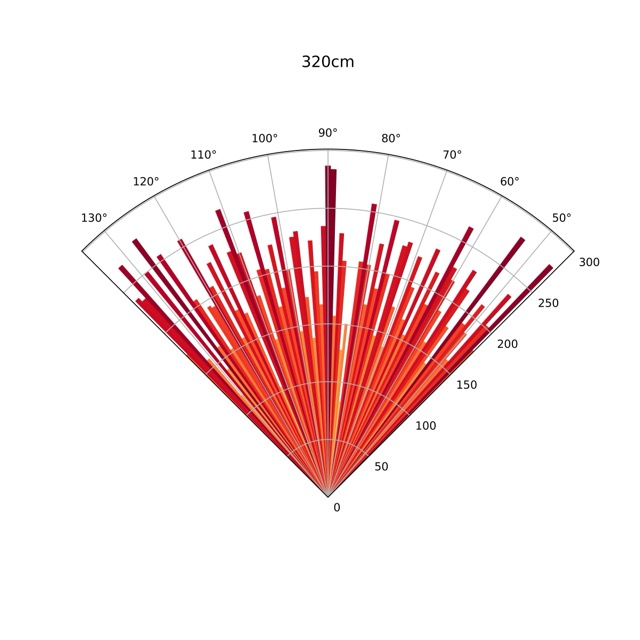
\includegraphics[width=\linewidth]{../Photos/angle-distance/320cm Medium}
  \end{subfigure}
  \label{fig:distance-angle3}
\end{figure}

\begin{figure}[H]
  \begin{subfigure}[b]{0.4\linewidth}
    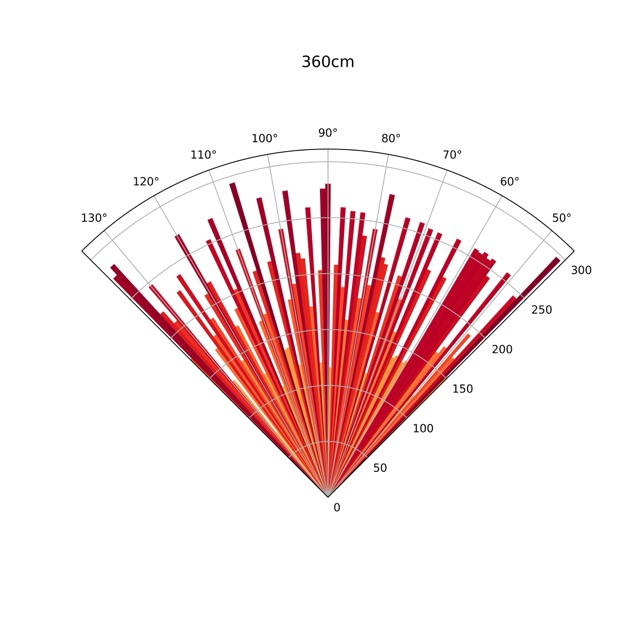
\includegraphics[width=\linewidth]{../Photos/angle-distance/360cm Medium}
  \end{subfigure}
  \hfill
  \begin{subfigure}[b]{0.4\linewidth}
    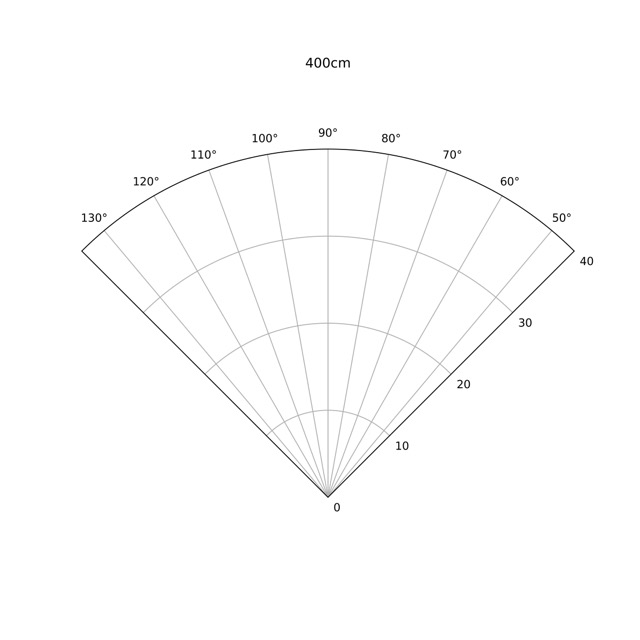
\includegraphics[width=\linewidth]{../Photos/angle-distance/400cm Medium}
  \end{subfigure}
  \label{fig:distance-angle4}
\end{figure}

\subsection{Code}
\textbf{Python Code of Black and White}
\begin{lstlisting}[language=Python]
import pandas as pd
import numpy as np
import matplotlib.pyplot as plt

file_paths = [f"./DataRestoration/{i}cm_0&1_data.xlsx" for i in range(0, 401, 40)]

distance_steps = np.arange(0, 401, 40)
angle_steps = np.arange(45, 136)
data_matrix = np.zeros((len(distance_steps), len(angle_steps)))

for idx, file_path in enumerate(file_paths):
    df = pd.read_excel(file_path)
    for _, row in df.iterrows():
        angle = int(row["Angle"])
        distance = row["Distance / cm"]
        if 45 <= angle <= 135:
            angle_idx = angle - 45
            data_matrix[idx, angle_idx] = distance

binary_matrix = np.where(data_matrix > 0, 1, 0)

angles = np.deg2rad(angle_steps)
distances = distance_steps
theta, r = np.meshgrid(angles, distances)

fig, ax = plt.subplots(subplot_kw={'projection': 'polar'}, figsize=(8, 8))

cmap = plt.cm.binary

heatmap = ax.pcolormesh(theta, r, binary_matrix, cmap=cmap, shading='auto')

ax.set_title("Radar Graph")

ax.set_thetamin(45)
ax.set_thetamax(135)
ax.set_rticks(distance_steps)
ax.set_rlabel_position(90)

plt.savefig("./Photos/RadarGraph.png", dpi=1200)
plt.show()
\end{lstlisting}

\textbf{Python Code of Data Average}
\begin{lstlisting}[language=Python]
import pandas as pd

file_paths = [
    "./DataProcessing/280cm/280cm_data_01.xlsx",
    "./DataProcessing/280cm/280cm_data_02.xlsx",
    "./DataProcessing/280cm/280cm_data_03.xlsx"
]

data_frames = [pd.read_excel(file) for file in file_paths]

combined_data = pd.concat(data_frames)
average_data = combined_data.groupby(combined_data.index).mean()

average_data = average_data.round(2)

output_file = "./DataAverage/280cm_average_data.xlsx"
average_data.to_excel(output_file, index=False)
\end{lstlisting}

\textbf{Python Code of Data Extraction}
\begin{lstlisting}[language=Python]
import pandas as pd

data_text = """
Angle: 135°; Distance: 218.58 cm
Angle: 134°; Distance: 274.31 cm
Angle: 133°; Distance: 0.00 cm
Angle: 132°; Distance: 0.00 cm
Angle: 131°; Distance: 188.98 cm
Angle: 130°; Distance: 248.95 cm
Angle: 129°; Distance: 309.20 cm
Angle: 128°; Distance: 42.93 cm
Angle: 127°; Distance: 117.10 cm
Angle: 126°; Distance: 179.23 cm
Angle: 125°; Distance: 236.17 cm
Angle: 124°; Distance: 299.51 cm
Angle: 123°; Distance: 357.11 cm
Angle: 122°; Distance: 85.48 cm
Angle: 121°; Distance: 161.19 cm
Angle: 120°; Distance: 220.33 cm
Angle: 119°; Distance: 280.51 cm
Angle: 118°; Distance: 336.40 cm
Angle: 117°; Distance: 63.27 cm
Angle: 116°; Distance: 138.78 cm
Angle: 115°; Distance: 207.50 cm
Angle: 114°; Distance: 265.57 cm
Angle: 113°; Distance: 329.91 cm
Angle: 112°; Distance: 57.25 cm
Angle: 111°; Distance: 126.04 cm
Angle: 110°; Distance: 179.61 cm
Angle: 109°; Distance: 255.90 cm
Angle: 108°; Distance: 307.29 cm
Angle: 107°; Distance: 0.00 cm
Angle: 106°; Distance: 0.00 cm
Angle: 105°; Distance: 219.49 cm
Angle: 104°; Distance: 288.14 cm
Angle: 103°; Distance: 338.66 cm
Angle: 102°; Distance: 69.89 cm
Angle: 101°; Distance: 142.47 cm
Angle: 100°; Distance: 200.50 cm
Angle: 99°; Distance: 268.19 cm
Angle: 98°; Distance: 348.21 cm
Angle: 97°; Distance: 358.93 cm
Angle: 96°; Distance: 163.18 cm
Angle: 95°; Distance: 243.96 cm
Angle: 94°; Distance: 323.93 cm
Angle: 93°; Distance: 65.22 cm
Angle: 92°; Distance: 150.85 cm
Angle: 91°; Distance: 239.12 cm
Angle: 90°; Distance: 317.81 cm
Angle: 89°; Distance: 55.74 cm
Angle: 88°; Distance: 152.36 cm
Angle: 87°; Distance: 56.66 cm
Angle: 86°; Distance: 65.03 cm
Angle: 85°; Distance: 56.99 cm
Angle: 84°; Distance: 65.03 cm
Angle: 83°; Distance: 56.53 cm
Angle: 82°; Distance: 69.47 cm
Angle: 81°; Distance: 0.00 cm
Angle: 80°; Distance: 0.00 cm
Angle: 79°; Distance: 0.00 cm
Angle: 78°; Distance: 0.00 cm
Angle: 77°; Distance: 0.00 cm
Angle: 76°; Distance: 0.00 cm
Angle: 75°; Distance: 0.00 cm
Angle: 74°; Distance: 0.00 cm
Angle: 73°; Distance: 0.00 cm
Angle: 72°; Distance: 0.00 cm
Angle: 71°; Distance: 0.00 cm
Angle: 70°; Distance: 0.00 cm
Angle: 69°; Distance: 0.00 cm
Angle: 68°; Distance: 0.00 cm
Angle: 67°; Distance: 0.00 cm
Angle: 66°; Distance: 0.00 cm
Angle: 65°; Distance: 0.00 cm
Angle: 64°; Distance: 0.00 cm
Angle: 63°; Distance: 0.00 cm
Angle: 62°; Distance: 66.78 cm
Angle: 61°; Distance: 56.65 cm
Angle: 60°; Distance: 65.36 cm
Angle: 59°; Distance: 64.43 cm
Angle: 58°; Distance: 63.90 cm
Angle: 57°; Distance: 59.25 cm
Angle: 56°; Distance: 56.78 cm
Angle: 55°; Distance: 57.21 cm
Angle: 54°; Distance: 15.80 cm
Angle: 53°; Distance: 56.78 cm
Angle: 52°; Distance: 196.09 cm
Angle: 51°; Distance: 287.76 cm
Angle: 50°; Distance: 56.80 cm
Angle: 49°; Distance: 115.88 cm
Angle: 48°; Distance: 197.79 cm
Angle: 47°; Distance: 275.62 cm
Angle: 46°; Distance: 0.00 cm
Angle: 45°; Distance: 0.00 cm
"""

data_lines = data_text.strip().split("\n")
extracted_data = []

for line in data_lines:
    parts = line.split(";")
    angle_part = parts[0].strip()
    distance_part = parts[1].strip()

    angle = int(angle_part.split(":")[1].strip().replace("°", ""))
    distance = float(distance_part.split(":")[1].strip().replace("cm", "").strip())

    extracted_data.append({"Angle": angle, "Distance / cm": distance})

df = pd.DataFrame(extracted_data)

df.to_excel("./DataProcessing/360cm/360cm_data_03.xlsx", index=False)
\end{lstlisting}

\textbf{Python Code of Graph Generate}
\begin{lstlisting}[language=Python]
import numpy as np
import pandas as pd
import matplotlib.pyplot as plt

file_name = "./DataAverage/280cm_average_data.xlsx"

df = pd.read_excel(file_name)
angles = df["Angle"].values
distances = df["Distance / cm"].values

valid_indices = distances > 0
angles = angles[valid_indices]
distances = distances[valid_indices]

theta = np.deg2rad(angles)

fig, ax = plt.subplots(subplot_kw={'projection': 'polar'}, figsize=(8, 8))

cmap = plt.cm.YlOrRd
vmin = 0
vmax = max(distances)
norm = plt.Normalize(vmin=vmin, vmax=vmax)
colors = cmap(norm(distances))

for i in range(len(theta)):
    ax.bar(
        theta[i],
        distances[i],
        width=np.deg2rad(1),
        color=colors[i],
        edgecolor="none",
        alpha=1.0
    )

sm = plt.cm.ScalarMappable(cmap=cmap, norm=norm)
sm.set_array([])

ax.set_title("280cm", va="bottom", fontsize=14)
ax.set_thetamin(45)
ax.set_thetamax(135)
ax.set_theta_zero_location("E")

plt.savefig("./Photos/angle-distance/280cm.png", dpi=1200)
plt.show()
\end{lstlisting}

\textbf{Python Code of Heatmap Generate}
\begin{lstlisting}[language=Python]
import pandas as pd
import mlx.core as mx
import matplotlib.pyplot as plt

file_paths = [f"./DataAverage/{i}cm_average_data.xlsx" for i in range(0, 401, 40)]

distance_steps = mx.arange(0, 400, 40)
angle_steps = mx.arange(45, 136)
data_matrix = mx.zeros((len(distance_steps), len(angle_steps)))

for idx, file_path in enumerate(file_paths):
    df = pd.read_excel(file_path)
    for _, row in df.iterrows():
        angle = int(row["Angle"])
        distance = row["Distance / cm"]
        if 45 <= angle <= 135:
            angle_idx = angle - 45
            data_matrix[idx, angle_idx] = distance

angles = mx.degrees(angle_steps)
distances = distance_steps
theta, r = mx.meshgrid(angles, distances)

fig, ax = plt.subplots(subplot_kw={'projection': 'polar'}, figsize=(8, 8))
cmap = plt.cm.Oranges
heatmap = ax.pcolor(theta, r, data_matrix, cmap=cmap, shading='auto')

cbar = plt.colorbar(
    heatmap,
    ax=ax,
    orientation='vertical',
    pad=0.1,
    shrink=0.6
)
cbar.set_label("Distance / cm", fontsize=12)

ax.set_title("Heatmap of \"Angle - Distance\"", va="bottom", fontsize=14)
ax.set_thetamin(45)
ax.set_thetamax(135)
ax.set_rticks(distance_steps)
ax.set_rlabel_position(90)

plt.savefig("./Photos/heatmap.png", dpi=1200)
plt.show()
\end{lstlisting}

\textbf{C code of Distance Detect}
\begin{lstlisting}[language=C++]
#include <Servo.h>
Servo engine;

// steering gear
int enginePin = 3;

// ultrasonic sensor
int ultrasound_TrigPin = 10;
int ultrasound_EchoPin = 11;

int counter = 0;

void setup() {
  // put your setup code here, to run once:
  Serial.begin(9600);
  // Engine Driver
  engine.attach(enginePin);
  // Ultrasound Driver
  pinMode(ultrasound_TrigPin, OUTPUT);
  pinMode(ultrasound_EchoPin, INPUT);
}

void loop() {
  // put your main code here, to run repeatedly:
  if(counter < 6) {
    engineTurn();
  } else if(engine.attached()) {
    engine.detach();
    Serial.println("STOP!!!");
  }
}

int angle = 90;
int step = 1;
unsigned long previousMillis = 0;

void engineTurn() {
  unsigned long currentMillis = millis();

  if(currentMillis - previousMillis >= 20) {
    previousMillis = currentMillis;

    engine.write(angle);

    ultrasoundControl();

    angle += step;

    // Change the direction when arrive the boundary
    if(angle >= 135) {
      angle = 135;
      step = -step;
      counter++;
    } else if(angle <= 45) {
      angle = 45;
      step = -step;
      counter++;
    }
  }
}

float duration, distance;

void ultrasoundControl() {
  digitalWrite(ultrasound_TrigPin, LOW);
  delayMicroseconds(2);
  digitalWrite(ultrasound_TrigPin, HIGH);
  delayMicroseconds(10);
  digitalWrite(ultrasound_TrigPin, LOW);

  duration = pulseIn(ultrasound_EchoPin, HIGH, 25000);
  distance = (duration * 0.0343) / 2;

  Serial.print("Angle: ");
  Serial.print(angle);
  Serial.print("°; Distance: ");
  Serial.print(distance);
  Serial.println(" cm");
}
\end{lstlisting}
